% Created by tikzDevice version 0.10.1 on 2016-05-08 18:26:50
% !TEX encoding = UTF-8 Unicode
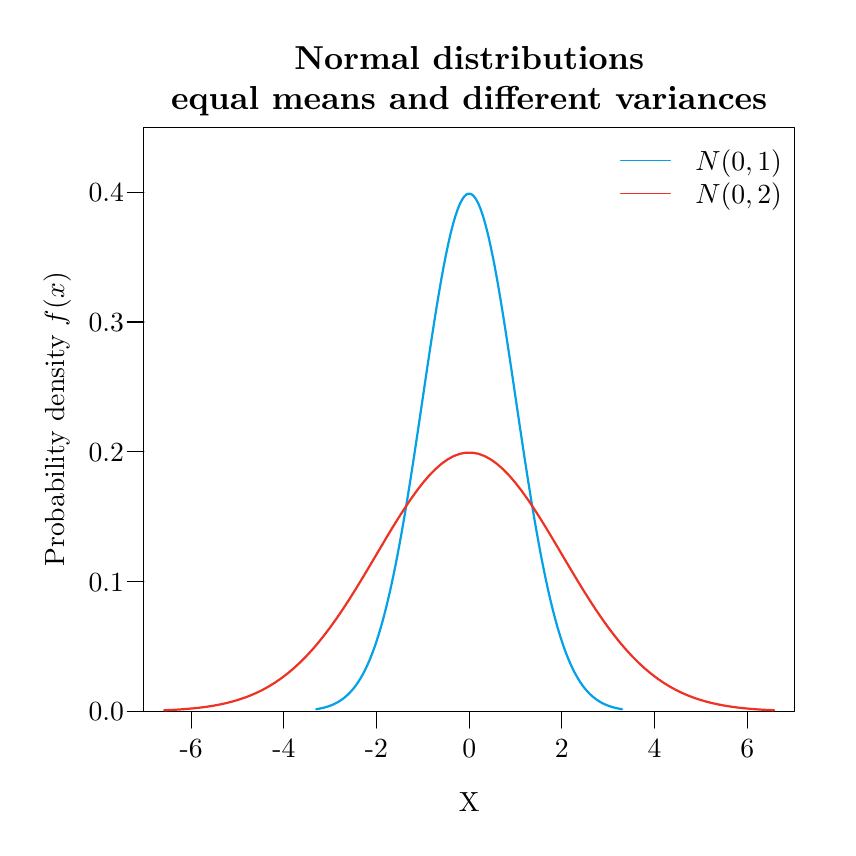
\begin{tikzpicture}[x=1pt,y=1pt]
\definecolor{fillColor}{RGB}{255,255,255}
\path[use as bounding box,fill=fillColor,fill opacity=0.00] (0,0) rectangle (289.08,289.08);
\begin{scope}
\path[clip] ( 42.00, 42.00) rectangle (277.08,253.08);
\definecolor{drawColor}{RGB}{5,161,230}

\path[draw=drawColor,line width= 0.8pt,line join=round,line cap=round] (104.29, 42.81) --
	(105.12, 42.95) --
	(105.96, 43.12) --
	(106.80, 43.31) --
	(107.63, 43.53) --
	(108.47, 43.79) --
	(109.31, 44.08) --
	(110.15, 44.41) --
	(110.98, 44.79) --
	(111.82, 45.22) --
	(112.66, 45.71) --
	(113.50, 46.27) --
	(114.33, 46.89) --
	(115.17, 47.59) --
	(116.01, 48.37) --
	(116.84, 49.25) --
	(117.68, 50.22) --
	(118.52, 51.31) --
	(119.36, 52.50) --
	(120.19, 53.83) --
	(121.03, 55.29) --
	(121.87, 56.89) --
	(122.70, 58.64) --
	(123.54, 60.55) --
	(124.38, 62.63) --
	(125.22, 64.89) --
	(126.05, 67.33) --
	(126.89, 69.95) --
	(127.73, 72.78) --
	(128.56, 75.80) --
	(129.40, 79.03) --
	(130.24, 82.47) --
	(131.08, 86.12) --
	(131.91, 89.97) --
	(132.75, 94.03) --
	(133.59, 98.29) --
	(134.42,102.75) --
	(135.26,107.40) --
	(136.10,112.23) --
	(136.94,117.23) --
	(137.77,122.38) --
	(138.61,127.67) --
	(139.45,133.09) --
	(140.28,138.60) --
	(141.12,144.19) --
	(141.96,149.83) --
	(142.80,155.50) --
	(143.63,161.17) --
	(144.47,166.81) --
	(145.31,172.39) --
	(146.15,177.88) --
	(146.98,183.25) --
	(147.82,188.47) --
	(148.66,193.50) --
	(149.49,198.30) --
	(150.33,202.86) --
	(151.17,207.14) --
	(152.01,211.11) --
	(152.84,214.74) --
	(153.68,218.01) --
	(154.52,220.90) --
	(155.35,223.37) --
	(156.19,225.43) --
	(157.03,227.04) --
	(157.87,228.20) --
	(158.70,228.90) --
	(159.54,229.13) --
	(160.38,228.90) --
	(161.21,228.20) --
	(162.05,227.04) --
	(162.89,225.43) --
	(163.73,223.37) --
	(164.56,220.90) --
	(165.40,218.01) --
	(166.24,214.74) --
	(167.07,211.11) --
	(167.91,207.14) --
	(168.75,202.86) --
	(169.59,198.30) --
	(170.42,193.50) --
	(171.26,188.47) --
	(172.10,183.25) --
	(172.93,177.88) --
	(173.77,172.39) --
	(174.61,166.81) --
	(175.45,161.17) --
	(176.28,155.50) --
	(177.12,149.83) --
	(177.96,144.19) --
	(178.80,138.60) --
	(179.63,133.09) --
	(180.47,127.67) --
	(181.31,122.38) --
	(182.14,117.23) --
	(182.98,112.23) --
	(183.82,107.40) --
	(184.66,102.75) --
	(185.49, 98.29) --
	(186.33, 94.03) --
	(187.17, 89.97) --
	(188.00, 86.12) --
	(188.84, 82.47) --
	(189.68, 79.03) --
	(190.52, 75.80) --
	(191.35, 72.78) --
	(192.19, 69.95) --
	(193.03, 67.33) --
	(193.86, 64.89) --
	(194.70, 62.63) --
	(195.54, 60.55) --
	(196.38, 58.64) --
	(197.21, 56.89) --
	(198.05, 55.29) --
	(198.89, 53.83) --
	(199.72, 52.50) --
	(200.56, 51.31) --
	(201.40, 50.22) --
	(202.24, 49.25) --
	(203.07, 48.37) --
	(203.91, 47.59) --
	(204.75, 46.89) --
	(205.58, 46.27) --
	(206.42, 45.71) --
	(207.26, 45.22) --
	(208.10, 44.79) --
	(208.93, 44.41) --
	(209.77, 44.08) --
	(210.61, 43.79) --
	(211.45, 43.53) --
	(212.28, 43.31) --
	(213.12, 43.12) --
	(213.96, 42.95) --
	(214.79, 42.81);
\end{scope}
\begin{scope}
\path[clip] (  0.00,  0.00) rectangle (289.08,289.08);
\definecolor{drawColor}{RGB}{0,0,0}

\path[draw=drawColor,line width= 0.4pt,line join=round,line cap=round] ( 59.08, 42.00) -- (260.00, 42.00);

\path[draw=drawColor,line width= 0.4pt,line join=round,line cap=round] ( 59.08, 42.00) -- ( 59.08, 36.00);

\path[draw=drawColor,line width= 0.4pt,line join=round,line cap=round] ( 92.57, 42.00) -- ( 92.57, 36.00);

\path[draw=drawColor,line width= 0.4pt,line join=round,line cap=round] (126.05, 42.00) -- (126.05, 36.00);

\path[draw=drawColor,line width= 0.4pt,line join=round,line cap=round] (159.54, 42.00) -- (159.54, 36.00);

\path[draw=drawColor,line width= 0.4pt,line join=round,line cap=round] (193.03, 42.00) -- (193.03, 36.00);

\path[draw=drawColor,line width= 0.4pt,line join=round,line cap=round] (226.51, 42.00) -- (226.51, 36.00);

\path[draw=drawColor,line width= 0.4pt,line join=round,line cap=round] (260.00, 42.00) -- (260.00, 36.00);

\node[text=drawColor,anchor=base,inner sep=0pt, outer sep=0pt, scale=  1.00] at ( 59.08, 25.20) {-6};

\node[text=drawColor,anchor=base,inner sep=0pt, outer sep=0pt, scale=  1.00] at ( 92.57, 25.20) {-4};

\node[text=drawColor,anchor=base,inner sep=0pt, outer sep=0pt, scale=  1.00] at (126.05, 25.20) {-2};

\node[text=drawColor,anchor=base,inner sep=0pt, outer sep=0pt, scale=  1.00] at (159.54, 25.20) {0};

\node[text=drawColor,anchor=base,inner sep=0pt, outer sep=0pt, scale=  1.00] at (193.03, 25.20) {2};

\node[text=drawColor,anchor=base,inner sep=0pt, outer sep=0pt, scale=  1.00] at (226.51, 25.20) {4};

\node[text=drawColor,anchor=base,inner sep=0pt, outer sep=0pt, scale=  1.00] at (260.00, 25.20) {6};

\path[draw=drawColor,line width= 0.4pt,line join=round,line cap=round] ( 42.00, 42.00) -- ( 42.00,229.63);

\path[draw=drawColor,line width= 0.4pt,line join=round,line cap=round] ( 42.00, 42.00) -- ( 36.00, 42.00);

\path[draw=drawColor,line width= 0.4pt,line join=round,line cap=round] ( 42.00, 88.91) -- ( 36.00, 88.91);

\path[draw=drawColor,line width= 0.4pt,line join=round,line cap=round] ( 42.00,135.81) -- ( 36.00,135.81);

\path[draw=drawColor,line width= 0.4pt,line join=round,line cap=round] ( 42.00,182.72) -- ( 36.00,182.72);

\path[draw=drawColor,line width= 0.4pt,line join=round,line cap=round] ( 42.00,229.63) -- ( 36.00,229.63);

\node[text=drawColor,anchor=base east,inner sep=0pt, outer sep=0pt, scale=  1.00] at ( 34.80, 38.56) {0.0};

\node[text=drawColor,anchor=base east,inner sep=0pt, outer sep=0pt, scale=  1.00] at ( 34.80, 85.46) {0.1};

\node[text=drawColor,anchor=base east,inner sep=0pt, outer sep=0pt, scale=  1.00] at ( 34.80,132.37) {0.2};

\node[text=drawColor,anchor=base east,inner sep=0pt, outer sep=0pt, scale=  1.00] at ( 34.80,179.28) {0.3};

\node[text=drawColor,anchor=base east,inner sep=0pt, outer sep=0pt, scale=  1.00] at ( 34.80,226.18) {0.4};

\path[draw=drawColor,line width= 0.4pt,line join=round,line cap=round] ( 42.00, 42.00) --
	(277.08, 42.00) --
	(277.08,253.08) --
	( 42.00,253.08) --
	( 42.00, 42.00);
\end{scope}
\begin{scope}
\path[clip] (  0.00,  0.00) rectangle (289.08,289.08);
\definecolor{drawColor}{RGB}{0,0,0}

\node[text=drawColor,anchor=base,inner sep=0pt, outer sep=0pt, scale=  1.20] at (159.54,274.09) {\bfseries Normal distributions};

\node[text=drawColor,anchor=base,inner sep=0pt, outer sep=0pt, scale=  1.20] at (159.54,259.69) {\bfseries  equal means and different variances};

\node[text=drawColor,anchor=base,inner sep=0pt, outer sep=0pt, scale=  1.00] at (159.54,  6.00) {X};

\node[text=drawColor,rotate= 90.00,anchor=base,inner sep=0pt, outer sep=0pt, scale=  1.00] at ( 13.20,147.54) {Probability density $f(x)$};
\end{scope}
\begin{scope}
\path[clip] ( 42.00, 42.00) rectangle (277.08,253.08);
\definecolor{drawColor}{RGB}{238,50,36}

\path[draw=drawColor,line width= 0.8pt,line join=round,line cap=round] ( 49.35, 42.42) --
	( 51.58, 42.52) --
	( 53.80, 42.64) --
	( 56.03, 42.79) --
	( 58.25, 42.97) --
	( 60.48, 43.18) --
	( 62.71, 43.43) --
	( 64.93, 43.73) --
	( 67.16, 44.08) --
	( 69.38, 44.50) --
	( 71.61, 44.98) --
	( 73.84, 45.54) --
	( 76.06, 46.19) --
	( 78.29, 46.93) --
	( 80.52, 47.78) --
	( 82.74, 48.75) --
	( 84.97, 49.84) --
	( 87.19, 51.07) --
	( 89.42, 52.45) --
	( 91.65, 53.98) --
	( 93.87, 55.68) --
	( 96.10, 57.55) --
	( 98.32, 59.60) --
	(100.55, 61.83) --
	(102.78, 64.24) --
	(105.00, 66.84) --
	(107.23, 69.62) --
	(109.45, 72.57) --
	(111.68, 75.69) --
	(113.91, 78.97) --
	(116.13, 82.39) --
	(118.36, 85.92) --
	(120.58, 89.56) --
	(122.81, 93.27) --
	(125.04, 97.03) --
	(127.26,100.80) --
	(129.49,104.55) --
	(131.71,108.25) --
	(133.94,111.86) --
	(136.17,115.34) --
	(138.39,118.65) --
	(140.62,121.76) --
	(142.84,124.63) --
	(145.07,127.23) --
	(147.30,129.52) --
	(149.52,131.47) --
	(151.75,133.07) --
	(153.97,134.28) --
	(156.20,135.10) --
	(158.43,135.51) --
	(160.65,135.51) --
	(162.88,135.10) --
	(165.11,134.28) --
	(167.33,133.07) --
	(169.56,131.47) --
	(171.78,129.52) --
	(174.01,127.23) --
	(176.24,124.63) --
	(178.46,121.76) --
	(180.69,118.65) --
	(182.91,115.34) --
	(185.14,111.86) --
	(187.37,108.25) --
	(189.59,104.55) --
	(191.82,100.80) --
	(194.04, 97.03) --
	(196.27, 93.27) --
	(198.50, 89.56) --
	(200.72, 85.92) --
	(202.95, 82.39) --
	(205.17, 78.97) --
	(207.40, 75.69) --
	(209.63, 72.57) --
	(211.85, 69.62) --
	(214.08, 66.84) --
	(216.30, 64.24) --
	(218.53, 61.83) --
	(220.76, 59.60) --
	(222.98, 57.55) --
	(225.21, 55.68) --
	(227.43, 53.98) --
	(229.66, 52.45) --
	(231.89, 51.07) --
	(234.11, 49.84) --
	(236.34, 48.75) --
	(238.56, 47.78) --
	(240.79, 46.93) --
	(243.02, 46.19) --
	(245.24, 45.54) --
	(247.47, 44.98) --
	(249.70, 44.50) --
	(251.92, 44.08) --
	(254.15, 43.73) --
	(256.37, 43.43) --
	(258.60, 43.18) --
	(260.83, 42.97) --
	(263.05, 42.79) --
	(265.28, 42.64) --
	(267.50, 42.52) --
	(269.73, 42.42);
\definecolor{drawColor}{RGB}{5,161,230}

\path[draw=drawColor,line width= 0.4pt,line join=round,line cap=round] (214.23,241.08) -- (232.23,241.08);
\definecolor{drawColor}{RGB}{238,50,36}

\path[draw=drawColor,line width= 0.4pt,line join=round,line cap=round] (214.23,229.08) -- (232.23,229.08);
\definecolor{drawColor}{RGB}{0,0,0}

\node[text=drawColor,anchor=base west,inner sep=0pt, outer sep=0pt, scale=  1.00] at (241.23,237.64) {$N(0,1)$};

\node[text=drawColor,anchor=base west,inner sep=0pt, outer sep=0pt, scale=  1.00] at (241.23,225.64) {$N(0,2)$};
\end{scope}
\end{tikzpicture}
